\chapter{Background Information and Literature}
\label{chap:background}

This chapter will introduce the necessary theory to understand \acrshort{fls}, its image formation process, and some \acrshort{fls} based approaches to registration.  

\section{Sonar Image Formation}

As is well explained by \citeauthor{noaaExplorationTools}\cite{noaaExplorationTools} and \citeauthor{Hurtos2015}\cite{Hurtos2015}, \acrfull{sonar}, sometimes also referred to as acoustic imaging, generate images using underwater sound waves. The \acrshort{sonar} contains in it an array of transducers that produce beams of acoustic waves in the water at different angles (bearings) and measure the time for it to "ping" or "echo" back. These sound waves travel across the water, reflecting off items like the bottom, underwater structures, and marine life. With this timing information, the system can generate detailed photos of the underwater world. This technology is widely utilized for navigation, mapping, and exploration, giving vital data for maritime research, underwater construction, and search and rescue operations.

Despite all of it's benefits and advantages, \acrshort{sonar} has a few pitfalls that specifically affect the goals of this thesis: 
\begin{itemize}
    \item According to \citeauthor{Hurtos2015}\cite{Hurtos2015}, the resulting images are often of low resolution, as compared to current camera technology. This is often a limitation of the medium as sound waves have a much higher wavelength than light. Higher-resolution images would offer more information and probably better-defined edges or areas of interest that would help the registration process.
    \item According to \citeauthor{Huang2020}\cite{Huang2020} sonar images tend to suffer from speckle noise: scattering and reverberation of the acoustic waves traveling through water results in a granular interference pattern that's typical of \acrshort{sonar} imaging. This is evidenced in the dark and bright spots often plaguing the image. Noise will undoubtedly introduce errors in the measurements, introducing uncertainty to the registrations. 
    \item It is susceptible to interference from other sources. For example, the onboard \acrshort{dvl} uses acoustic beams to measure the velocity of the vehicle relative to the seafloor, which can create signal interference with the sonar system, potentially leading to degraded image quality or inaccurate data. This interference might lead to inaccurate registrations which might affect the resulting output image.
\end{itemize}


The number of beams produced by the sonar and their orientation will determine the sonar's angular resolution and field of view:
\begin{figure}[H]
    \centering
    \begin{subfigure}[b]{.35\textwidth}
        \centering
        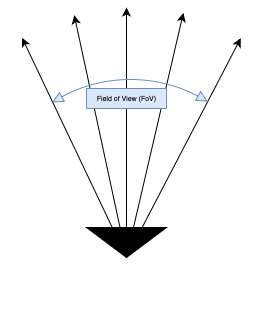
\includegraphics[width=\textwidth]{figures/FLS-TopView.png}
        \caption{Top-view of the sonar showing how all the beams spread out from the device.}
        \label{fig:flstop}
    \end{subfigure}
    \hfill
    \begin{subfigure}[b]{.55\textwidth}
        \centering
        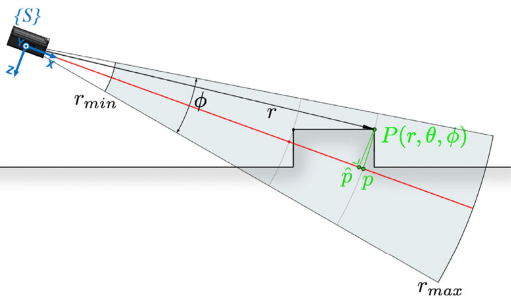
\includegraphics[width=\textwidth]{figures/FLS.png}
        \caption{Side-view of the sonar showing the effect of the \acrshort{fls} vertical aperture. Image created by \citeauthor{Hurtos2015} \cite{Hurtos2015}.}
        \label{fig:flsaperture}
    \end{subfigure}
    \caption{Top and side views of the sonar beams. In the side-view image, only one beam coming from the sonar is shown.}
\end{figure}


As explained by \citeauthor{Hurtos2015}\cite{Hurtos2015}, in \acrfull{fls} imaging, a particular beam generated from the transducer might spread along its "Vertical Aperture". All the pings along the aperture arc get compacted down into the image plane. In a similar fashion to what happens in a regular optical camera, a 2D \acrfull{fls} loses 3D information of the captured scene. Any set of points above or below the image plane along the same arc will correspond to the same output in the sonar image. The figure \ref{fig:flsaperture} shows a single beam coming from the sonar and how it is mapped into a single vertical line in the output image. Any echoes received back from insonifying this cone will be mapped onto the red "imaging plane", generating the loss of 3D data. 

Although the 3D point \(P\) actually matches the point \(p\) on the imaging plane, as long as the range is much greater than the relief observed in the elevation direction we can approximate the 3D point \(P\) to \(\hat{p}\). This is often the case as on \acrshort{fls} the vertical aperture tends to be small, and ranges can extend very far.


\subsection{Fan Transformation}
\label{sec:fan-tform}
\begin{figure}[H]
    \centering
    \begin{subfigure}[b]{.45\textwidth}
        \centering
        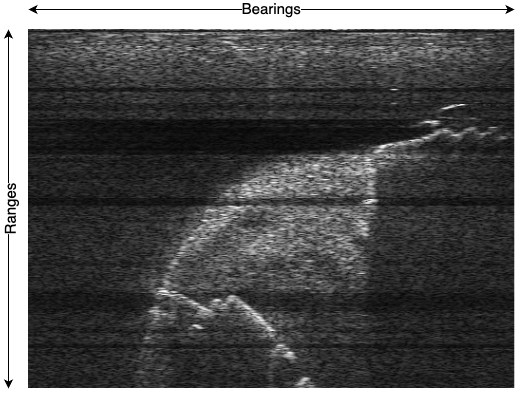
\includegraphics[width=\textwidth]{figures/sonar_raw_annotated.png}
        \caption[\acrshort{fls} raw data]{Raw data obtained from the sonar}
        \label{sfig:sonarraw}
    \end{subfigure}
    \hfill
    \begin{subfigure}[b]{.45\textwidth}
        \centering
        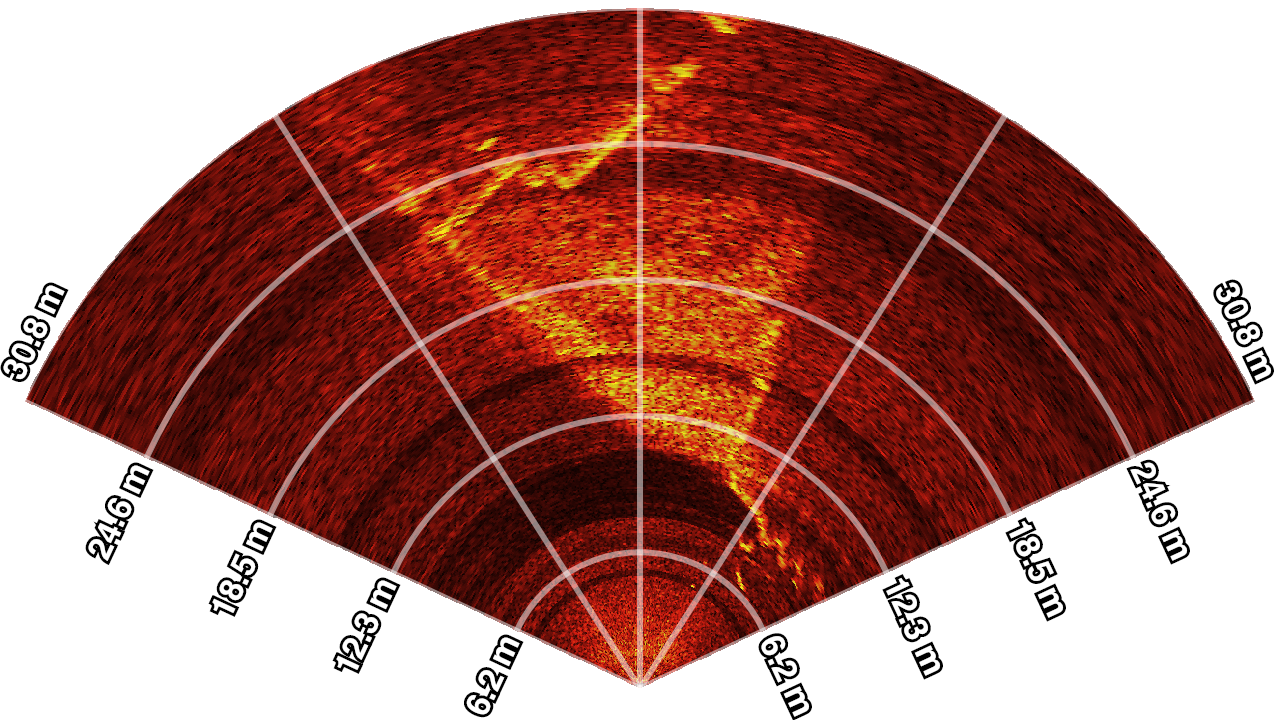
\includegraphics[width=\textwidth]{figures/sonar_processed.png}
        \caption{Processed \acrshort{fls} data}
        \label{sfig:sonarfan}
    \end{subfigure}
    \caption{Using the data from the bearing table we can transform the raw data into actual sonar images.}
\end{figure}

From the sonar driver code and its resources \cite{Blueye:OculusDriver} a few things become clear. The raw data from the sensor is structured in an array that represents ping intensity at a specific bearing and range. It is important to note that the beam bearings are not evenly spaced. The sensor provides a bearing table that accompanies the frame with the specific angle associated with each beam. Using this information we can create a mapping \(F(u,v)=I(\theta,r)\) that will produce pixel values for the output fan image based on the bearing and range from the source image. For any \((u,v)\) pair in the output fan image, we can calculate the corresponding \((\theta, r)\) from the source image. Looking only at the output image, we see that the mapping from \((\theta, r)\) to \((u, v)\) boils down to simple trigonometry. The output image will have the same height (\(H\)) as the input image, i.e. the number of ranges. The width will be limited by the maximum and minimum bearing angle and the height of the image. It can be calculated as follows: 

\begin{equation}
    W = 2 * H * \sin{\frac{FOV}{2}} 
\end{equation}

There are a couple of considerations to keep in mind:
\begin{itemize}
    \item The top row of the raw image \ref{sfig:sonarraw} has index 0. Since the output image \ref{sfig:sonarfan} expects the origin of the rays to be at the bottom, the image must be flipped. This can be achieved by replacing the y-coordinate \(v\) with \(H - v\), where \(H\) is the height of the images (the number of ranges).
    \item The angle \(\theta\) is measured between the beam in question and the y-axis of the output fan image. This axis is centered in the image as in \ref{sfig:sonarfan}. To center the coordinate frame, the x-coordinate \(u\) is replaced with \((u - W / 2)\), where W is the width of the output image.
    \item Any mapping that results in a value of \(r\) beyond the number or ranges in the source image is invalid, i.e. \(r \in [ 0, maxRange ]\). The same goes for values of theta that are outside of the range of the bearing table, i.e. \(\theta \in [ -minBearing, maxBearing] \). In any of these cases, the resulting pixel will be outside of the fan.
\end{itemize}


\[
\theta = \arctan(\frac{u - W / 2}{ H - v}))
\]
\[
r = \sqrt{(u - W / 2) ^ 2 + (H - v)^ 2}
\]

The value of \(r\) will represent then the y-axis coordinate in the source image (the "Ranges" axis). It is necessary to round it to the closest integer to access the pixel value. The value of \(\theta\) can be linked to its corresponding index along the x-axis of the source image through the bearing table. The index of the closest value to \(\theta\) will represent the coordinate on the "Bearings" axis.

\section{Speedup}
\label{sec:speedup}

Speedup is a metric that will be used to evaluate some of the results. It is a measure of the relative performance of two systems evaluating the same problem \cite{enwiki:1225834080}:

\[S_{latency} = \frac{L_{old}}{L_{new}}\]


\section{Mosaicing}
\label{sec:mosaicing}


According to \citeauthor{Capel2001}\cite{Capel2001}:
\begin{quote}
\textit{Image mosaicing is the alignment of multiple images into larger compositions which represent portions of a 3D scene. It generally applies to images related by planar homographies.}
\end{quote}

According to \citeauthor{Capel2001}, homographies can be estimated from images in two cases:
\begin{itemize}
    \item \textbf{Images of planes:} images taken from different viewpoints of a fully planar surface.
    \item \textbf{Rotation about the camera center}: images taken as the camera rotates about its center. The scene is allowed to be 3D in this case.
\end{itemize}

If the range that the sonar images are taken from is much larger than whatever variation in depth there is at the seabed, we can approximate our system as taking images of a planar surface in which case traditional mosaicing techniques would apply. 

Using the techniques that will be described in the following sections it will be possible to estimate these homographies between consecutive frames. What's left after that is implementing an algorithm that would combine the data from all the frames using the estimated homographies.

Combining the images is a topic in itself. There are many considerations like the best way to blend the seams, the best way to reduce noise, super-sampling, etc. A simple approach, but quite effective against speckle noise is averaging the overlapping part of the images. Since the noise and the underlying signal have a low correlation, averaging the images results in a noise-attenuating effect. Ideally, this reduction of noise is proportional to the squared number of average samples \cite{Hurtos2015}. For example, to cut the noise in half in the area of the mosaic, four overlapping images would be required. 
% \section{\acrfull{dvl}}

\section{Registration in the Frequency Domain}

"Registration in the frequency domain" describes methods that often use the Fourier transform to estimate the transformation between two images. They are often based on properties of the \acrfull{fft}, and offer several advantages that are of interest to the registration of sonar images:
\begin{itemize}
    \item Robustness to noise: Frequency domain methods, especially when using phase correlation, are relatively robust to noise and intensity variations\cite{Reddy1996}.
    \item Frequency domain methods can be extended to handle not just translations, but also rotations and scaling \cite{Reddy1996}.
    \item Low computational complexity of the \acrshort{fft}:  \(O(N\log_2N)\)\cite{Haynal2011}. Fast and inexpensive methods are preferred so as to not restrict where the algorithm might run. This could allow the \acrshort{rov} to execute the algorithm on a much more limited CPU.
\end{itemize}

Robustness to noise in particular is of interest when developing registration pipelines for sonar images. As mentioned before, sonar images are very noisy. Feature-based algorithms might mistake the noise as relevant image information which would be undesirable.

\subsection{Phase Correlation}

The phase correlation method allows us to estimate translations between images using the Fourier transform. By converting the images into the frequency domain, the method identifies shifts as phase differences between their corresponding Fourier transforms. The resulting phase correlation peak indicates the relative translation between the images, providing a robust and efficient way to align them even in the presence of noise or varying image intensities. It uses a property called Fourier shift which relates translations in the spatial domain to phase shifts in the Fourier domain. 


Better explained by \citeauthor{Reddy1996}\cite{Reddy1996} and \citeauthor{5396234}\cite{5396234}, the process of identifying the translation between two images is as follows. Given two images \(f_1\) and \(f_2\) related by a translation in the x and y axis, \(t_x\) and \(t_y\) respectively:

\[f_2(x,y)=f_1(x-t_x,y-t_y)\]

When converted to the Fourier domain:

\[F_2(\xi,\eta)=e^{-j2\pi(\xi t_x + \eta t_y)} F_1(\xi,\eta)\]

It can be concluded that the Fourier transform of each image is the same in magnitude, but has a phase shift given by \(e^{-j2\pi(\xi t_x + \eta t_y)}\). The shift theorem guarantees that the phase of the cross-power spectrum is equivalent to the phase difference between the images. Using the normalized \acrfull{cps} we can calculate this phase shift:

\[e^{-j2\pi(\xi t_x + \eta t_y)} = \frac{F_1(\xi,\eta) \; F_2^*(\xi,\eta)}{|F_1(\xi,\eta) \; F_2(\xi,\eta)|}\]

Computing the inverse Fourier transform of the \acrshort{cps} returns an impulse function, i.e. mostly zeros everywhere except for a peak/impulse. This is also called a dirac delta function. The coordinates of this peak represent the shifts \(t_x\) and \(t_y\).

Although this is a great building block for the registration pipeline, it has the limitation of only being able to detect translations. The images that will be captured in the sonar will also experience rotations which makes this method, by its own, useless. This is where the next point, the polar and log-polar transforms come in.

\subsection{Polar Transforms}

The polar transform in this context is used to to convert from a 2D cartesian coordinate system to 2D polar coordinate system. Coordinates typically expressed in \((x, y)\), are represented by radius and angle \((\rho, \theta)\) as measured from the image center \((x_x, y_c)\):

\[\rho = \sqrt{(x-x_c)^2 + (y - y_c)^2}\]
\[\theta = \arctan{\frac{y - y_c}{x-x_c}}\]

This brings rise to a useful property: rotations in the cartesian coordinate system are represented by shifts in the $\theta$ axis of its polar counterpart.

Recalling the structure of the images provided by the sonar, this sounds very familiar. Indeed, the raw sonar frames are a polar representation of the scene. 

There is still one more issue that a regular polar transform can't account for: scaling of the images. According to \citeauthor{5396234}\cite{5396234}, in a log-polar transform scaling is represented by a shift in the $\rho$ axis:

\[\rho = \log(\sqrt{(x-x_c)^2 + (y - y_c)^2}\]
\[\theta = \arctan{\frac{y - y_c}{x-x_c}}\]

Knowing that we can use phase correlation to identify translations in images, a combination of a polar transform and phase correlation might help us then identify the rotation between the images. This is what the Fourier-Mellin approach proposes.

\section{Fourier-Mellin Registration Pipeline}
\label{sec:fm-registration}

The Fourier-Mellin registration pipeline takes advantage of a second property of the Fourier transform of two images in the case when they are rotated. Again \citeauthor{Reddy1996}\cite{Reddy1996} explains it in simple terms. Given two images \(f_1\) and \(f_2\) related by a translation \(t_x\) and \(t_y\) and a rotatation \(\theta\):

\[f_2(x,y)=f_1(x \cos{\theta} + y \sin{\theta} -t_x, - x \sin{\theta} + y \cos{\theta} - t_y)\]

When converted to the Fourier domain:

\[F_2(\xi,\eta)=e^{-j2\pi(\xi t_x + \eta t_y)} F_1(\xi\cos{\theta} + \eta\sin{\theta},-\xi\sin{\theta} + \eta\cos{\theta})\]

Ignoring the phase and only working with the polar representation of the magnitudes, rotational movement \(\theta_0\) decoupled from translations can be deduced by using phase correlation.

\[M_2(\xi,\eta)=M_1(\xi\cos{\theta} + \eta\sin{\theta},-\xi\sin{\theta} + \eta\cos{\theta})\]
\[\mbox{Converting to polar representation, }M_2(\rho,\theta)=M_1(\rho,\theta - \theta_0)\]
\[\mbox{Applying phase correlation and identifying peak} \rightarrow \theta_0\]

This can be extended to account for scaling differences using the log-polar transform. This process is also used by \citeauthor{5396234}\cite{5396234} to register medical images, which are generated in a similar fashion to sonar. In this case, when applying phase correlation, the coordinates of the peak will represent both scaling and rotation.

In essence the Fourier-Mellin Pipeline does the following:

\begin{itemize}
    \item Apply the Discrete Fourier Transform (DFT) to shift images into the frequency domain.
    \item Use smoothing and high-pass filtering to prevent border-induced artifacts and reduce aliasing artifacts caused by rotation.
    \item Perform a log-polar transform to map rotation and scaling in Cartesian coordinates to translations in the log-polar coordinate system.
    \item Use Phase Correlation to determine the translation offset between two images. This yields rotation.
    \item Apply this rotation to the original image.
    \item Use Phase Correlation again over the rotated image to identify translation.
\end{itemize}

The most attractive factor of this approach is that it can decouple the rotation of the image from its translation. On simulated data, it is possible to achieve perfect rotations and perfect translations, but when using data from a sonar mounted to the \acrshort{rov}, the frames will experience both rotation and translation at the same time from the smallest perturbations, even if the sonar is trying not to move, or trying to only rotate or translate in one direction.


\section{\citeauthor{Hurtos2015}'s Raw Polar Registration Pipeline}

\begin{figure}[H]
  \centering
  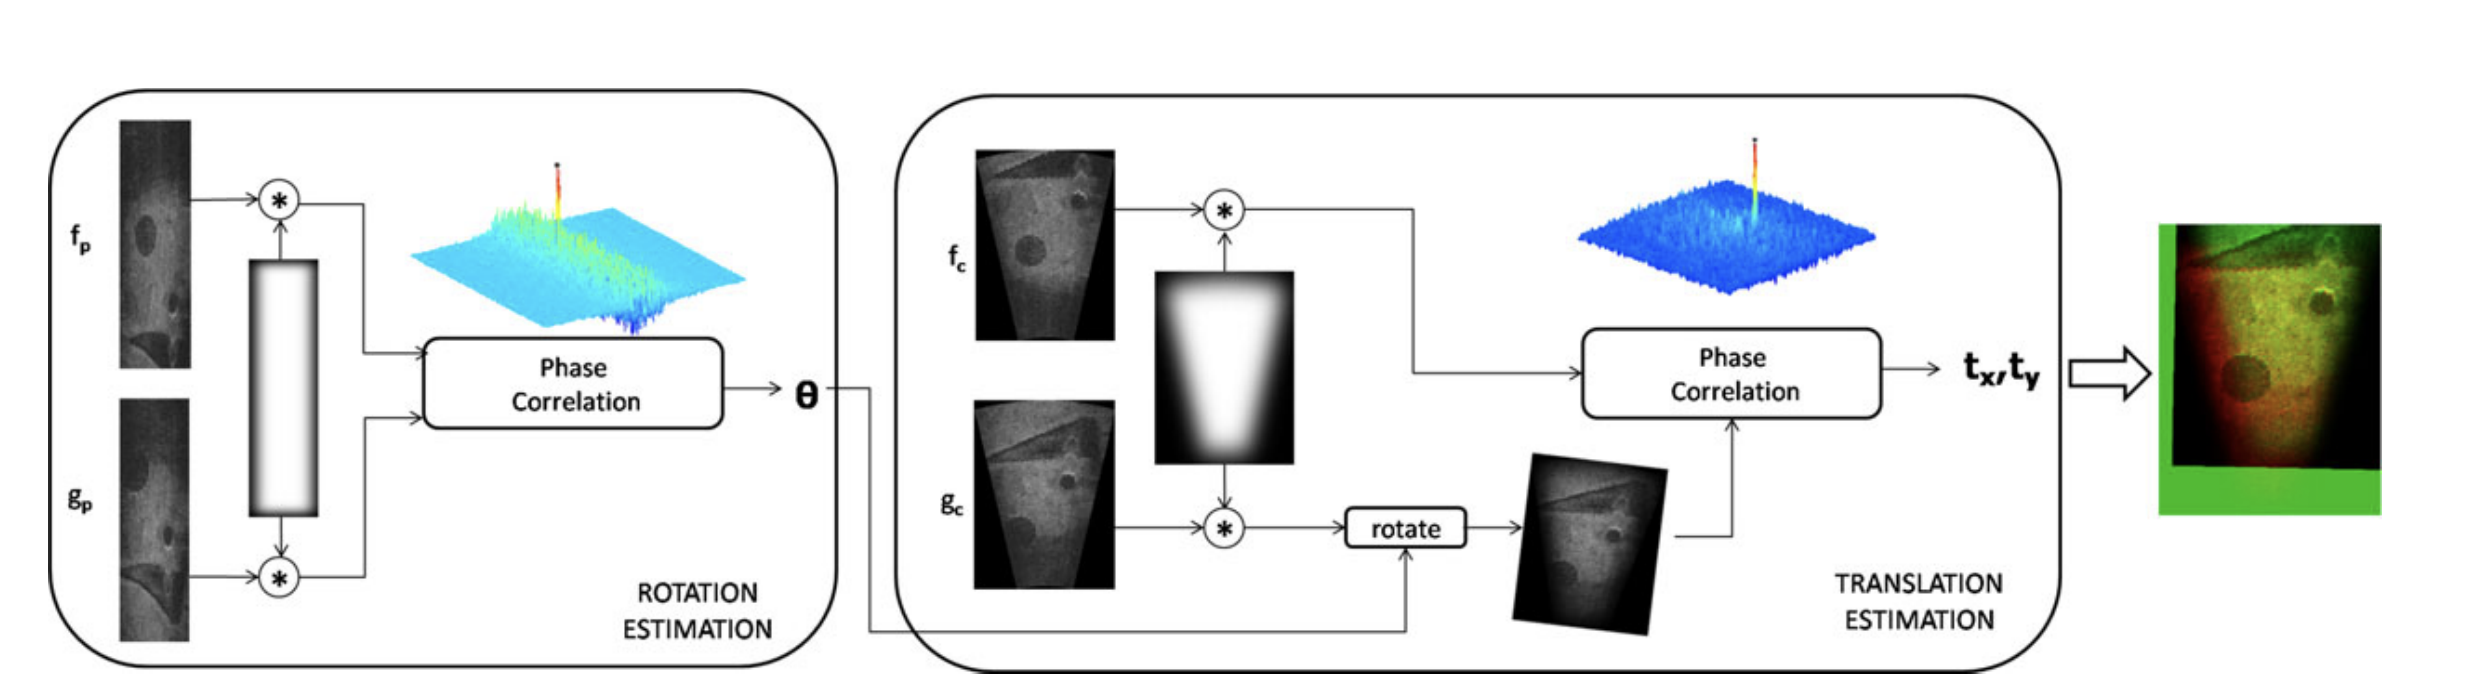
\includegraphics[width=\textwidth]{figures/RawPolarPipeline.png}
  \caption{Raw Polar Registration Pieline. Image created by \citeauthor{Hurtos2015}\cite{Hurtos2015}.}
  \label{fig:raw-polar-pipeline}
\end{figure}


\citeauthor{Hurtos2015} proposes a shorter pipeline than the Fourier-Mellin approach. Instead of estimating the rotation using the Log-Polar transform of the images in Fourier domain, it proposes using Phase Correlation over the raw sonar frames. Because of this, the pipeline will be referred to through the text as the "Raw Polar Pipeline". Since the input frames are already in a polar representation of sorts, given a short enough displacement between the two frames they claim it is possible to estimate the rotation angle directly.

As can be seen in \autoref{fig:raw-polar-pipeline}, this pipeline is very simple. It calculates rotation on two masked raw sonar frames using Phase Correlation. Using the estimated rotation, it proceeds to apply the Fan Transformation over the inputs, masking them with a blurred fan-shaped mask, and warps the second frame using the estimated angle. Using phase correlation again, the translation can be estimated.

The authors mention that instead of trying to filter out the noise, they would keep it throughout the pipeline and rely on global alignment to fix any errors. Since global alignment won't be part of the focus of the thesis, the implementation of this pipeline will include some filtering after the Fan Transformation, following recommendations from \citeauthor{5396234}\cite{5396234} and \citeauthor{Reddy1996}\cite{5396234}.